% Preamble
% ---

% These are the instructions for authors for IJCAI-18.
% They are the same as the ones for IJCAI-11 with superficical wording
%   changes only.

\documentclass{article}
\usepackage{icml2018}
\usepackage{times}  %Required
\usepackage{helvet}  %Required
\usepackage{courier}  %Required
\usepackage{url}  %Required
\usepackage{graphicx}  %Required
\usepackage{titlesec}
\usepackage{mathtools}
\usepackage{comment}
\usepackage[11pt]{moresize}

\usepackage{graphicx}

\makeatletter
\newcommand*\bigcdot{\mathpalette\bigcdot@{.5}}
\newcommand*\bigcdot@[2]{\mathbin{\vcenter{\hbox{\scalebox{#2}{$\m@th#1\bullet$}}}}}
\makeatother

\frenchspacing  %Required
\setlength{\pdfpagewidth}{8.5in}  %Required
\setlength{\pdfpageheight}{11in}  %Required
\setcounter{secnumdepth}{2}  
 
\titlespacing*{\paragraph}{0pt}{1.5ex plus 1ex minus .2ex}{1.3ex plus .2ex}
 
\usepackage{times}
\usepackage{xcolor}
\usepackage{soul}
%\usepackage[small]{caption}
\usepackage{nicefrac}
\usepackage{mathtools}

\usepackage{graphicx}
\usepackage{subfig}
\usepackage{caption}
% Packages
% ---
\usepackage{amsmath} % Advanced math typesetting
\usepackage{amssymb}
\usepackage{amsthm}
\usepackage{mathabx}
\usepackage{array}
\usepackage{bbm}
%\usepackage{subcaption}
\usepackage[ruled,linesnumbered,vlined]{algorithm2e}
%\usepackage{tikz}
%\usepackage{tkz-graph}
\usepackage{calrsfs}
%\usetikzlibrary{shapes,arrows,positioning,calc}
\usepackage[capitalize]{cleveref}

% control space before and after plot/image
\usepackage[belowskip=-5pt,aboveskip=5pt]{caption}
\setlength{\intextsep}{10pt plus 2pt minus 2pt} %distance between floats inserted inside the page text (using h) and the text proper.
\setlength{\textfloatsep}{10pt plus 2pt minus 2pt} %distance between floats on the top or the bottom and the text;
\setlength{\floatsep}{10pt plus 2pt minus 2pt} %distance between two floats;

\usepackage{tkz-graph}
\usepackage{tikz}
\usetikzlibrary{arrows,automata,positioning}
%\GraphInit[vstyle = Shade]
\tikzset{
	LabelStyle/.style = {minimum width = 1em, fill = white!50, opacity=0.8,
		text = black, font = \tiny },
	VertexStyle/.append style = { inner sep=2pt,
		font = \bfseries},
	EdgeStyle/.append style = {->, bend left} }

\crefname{algocf}{Algorithm}{Algorithm}
\Crefname{algocf}{Algorithm}{Algorithm}

\DeclarePairedDelimiter{\ceil}{\lceil}{\rceil}
\DeclarePairedDelimiter{\norm}{\lVert}{\rVert}
\DeclarePairedDelimiter{\abs}{\vert}{\rvert}

\makeatletter
\newcommand{\citeasnoun}[1]{\cite{#1}}
\newcommand*{\rom}[1]{\expandafter\@slowromancap\romannumeral #1@}
\makeatother
\newcommand{\E}{\mathbb{E}}
\renewcommand{\P}{\mathbb{P}}
\newcommand{\setsep}{~:~}
\newcommand{\opt}{^\star}
\newenvironment{mprog}{\begin{array}{>{\displaystyle}l>{\displaystyle}l>{\displaystyle}l}}{\end{array}}
\newcommand{\stc}{\\[1ex]  \mbox{s.t.} &}
\newcommand{\cs}{\\[1ex] & }
\newcommand{\minimize}[1]{\min_{#1} &}
\newcommand{\maximize}[1]{\max_{#1} &}
\newcommand{\tr}{^{\mathsf{T}}}
\newcommand{\one}{\mathbf{1}}
\newcommand{\Real}{\mathbb{R}}
\renewcommand{\ss}{~:~}

\newcommand{\eye}{\mathbf{I}}
\newcommand{\zero}{\mathbf{0}}

\usepackage{natbib}
\bibliographystyle{named}
\setcitestyle{square}

\newcommand{\RNum}[1]{\uppercase\expandafter{\romannumeral #1\relax}}
\newcommand*{\todo}{\textcolor{red}}
\newcommand{\marek}[1]{\textcolor{blue}{[[#1]]}}

\newcommand{\states}{\mathcal{S}}
\newcommand{\actions}{\mathcal{A}}
\newcommand{\mdp}{\mathcal{M}}
\newcommand{\data}{\mathcal{D}}
\newcommand{\pset}{\mathcal{P}}
\newcommand{\tran}{p\opt}
\newcommand{\aset}{\mathcal{P}}
\newcommand{\aseth}{\aset^{H}}
\newcommand{\asetht}{\aset^{T}}
\newcommand{\asetb}{\aset^{B}}
\newcommand{\asetr}{\aset^{R}}
\newcommand{\BU}{T}
\newcommand{\rob}{^R}
\newcommand{\RBU}{\widehat{T}}
\newcommand{\indicator}{\mathbbm{1}}
\newcommand{\vset}{\mathcal{V}}
\newcommand{\vsetr}{\vset^R}

\newcommand{\statecount}{S}
\newcommand{\actioncount}{S}

%\newcommand{\fix}[1]{}
\newcommand{\fix}[1]{{$\langle${\color{red}\sc Fix: #1}$\rangle$}}

\theoremstyle{plain}
\newtheorem{theorem}{Theorem}[section]
\newtheorem{corollary}[theorem]{Corollary}
\newtheorem{lemma}[theorem]{Lemma}
\newtheorem{proposition}[theorem]{Proposition}
\theoremstyle{definition}
\newtheorem{definition}[theorem]{Definition}

\title{Robust Exploration with Tight Bayesian Plausibility Sets}
%PDF Info Is Required:
\pdfinfo{
	/Tight Bayesian Ambiguity Sets for Robust MDPs
	/author names}

\author{
UNH
}
\date{}
% Main document
% ---
\begin{document}
\maketitle

%\tikzset{
%block/.style = {draw, fill=white, rectangle, minimum height=3em, minimum width=3em},
%tmp/.style  = {coordinate}, 
%sum/.style= {draw, fill=white, circle, node distance=1cm},
%input/.style = {coordinate},
%output/.style= {coordinate},
%pinstyle/.style = {pin edge={to-,thin,black}}
%}

\begin{abstract}
Optimism about the poorly understood states and actions is the main driving force of exploration for many provably-efficient reinforcement learning algorithms. We propose optimism in the face of sensible value functions (OFVF)- a novel reinforcement learning algorithm designed to explore robustly minimizing the worst case exploration cost. OFVF proceeds in an episodic manner, where the duration of the episode is fixed and known. OFVF relaxes the requirement for the set of plausible MDPs to be represented by a confidence interval. It also optimizes the size and location of the plausibility set. Our algorithm is inherently Bayesian and can leverage prior information. Our theoretical analysis shows the robustness of OFVF, and the empirical results demonstrate its practical promise.
\end{abstract}

\section{Introduction}

Markov decision processes (MDPs) provide a versatile methodology for modeling dynamic decision problems under uncertainty~\citep{Bertsekas1996,Sutton1998,Puterman2005}. A perfect MDP model for many reinforcement learning problems is not known precisely in general. Instead, a reinforcement learning agent tries to maximize its cumulative payoff by interacting in an unknown environment with an effort to learn the underlying MDP model. It is important for the agent to explore
sub-optimal actions to accelerate the MDP learning task which can help to optimize long-term performance. But it is also important to pick actions with highest known rewards to maximize short-run performance. So the agent always needs to balance between them to boost the performance of a learning algorithm during learning. 

\emph{Optimism in the face of uncertainty (OFU)} is a common principle for most reinforcement learning algorithms encouraging exploration~\citep{Jaksch2010,Brafman2001,Kearns1998a}. The idea is to assign a very high exploration bonus to poorly understood states and actions. The agent chooses a policy under this very "optimistic" model of the environment. As the less understood states-actions are incentivized, they seem lucrative to the agent encouraging exploration. As the agent visits and gathers statistically significant evidence for these states-actions, the uncertainty and optimism decreases converging to reality. Many RL algorithms including \emph{Explicit Explore or Exploit $(E^3)$}~\citep{Kearns1998a}, \emph{R-{\ssmall MAX}}~\cite{Brafman2001}, \emph{UCRL2}~\cite{Auer2006}, \emph{MBIE}~\citep{Strehl2008,Strehl2004,Wiering1998} build on the idea of optimism guiding the exploration. These algorithms provide strong theoretical guarantees with polynomial bound on sample complexity. 

The performance of these OFU algorithms greatly depends on the methods to implement optimism (e.g. Chernoff-Hoeffding's inequality for UCRL2, Confidence Interval for MBIE), which can often be complex in nature. Dealing with a family of plausible environments can sometimes become expensive as well. With OFU exploration, it is possible for an agent to be overly optimistic about a potentially catastrophic situation and end up there paying an extremely high price (e.g. a self driving car hits a wall, a robot falls off the cliff etc.). Exploring and learning such a situation may not payoff the price. It can be wise for the agent to be robust and avoid those situations minimizing the worst-case exploration cost$-$ which we call robust exploration. OFU algorithms are optimistic by definition and cannot guarantee robustness while exploring.

\emph{Probability matching} class of algorithms like \emph{Thompson sampling}~\citep{Thompson1933} performs exploration with a proportional likelihood to the underlying true parameters and has been successfully applied to multi-armed bandit problems~\citep{Agrawal2012,Agrawal2011}. \emph{Posterior Sampling for reinforcement learning (PSRL)}~\citep{Osband2016, Osband2013, Strens2002} applies the same idea in the context of reinforcement learning. PSRL algorithm samples a single instance of the environment from the posterior distribution, then solves and executes the policy optimal for that sampled environment over the episode. Selection of a policy in PSRL is proportional to the probability of that being optimal and exploration is guided by the variance of sampled policies as opposed to optimism. PSRL algorithm is simple, computationally efficient and can utilize any prior structural information to improve exploration. Strong theoretical analysis and practical applications for PSRL are also established in the literature. But similar to OFU algorithms, PSRL cannot handle worst case exploration penalty and performs poorly in such situations.

The main contribution of this paper is OFVF, a new \emph{data-driven} Bayesian approach to constructing \emph{Plausibility} sets for MDPs. The method computes policies with tighter robust estimates for exploration by introducing two new ideas. First, it is based on Bayesian posterior distributions rather than distribution-free bounds. Second, OFVF does not construct plausibility sets as simple confidence intervals. Confidence intervals as plausibility sets are a sufficient but not a necessary condition. OFVF uses the structure of the value function to optimize the \emph{location} and \emph{shape} of the plausibility set to guarantee upper bounds directly without necessarily enforcing the requirement for the set to be a confidence interval.

The paper is organized as follows: \cref{sec:prbolem} formally defines the problem setup and goals of the paper. \cref{sec:IE} reviews some existing methods to construct the plausibility sets and their extension to Bayesian setting. OFVF is proposed and analyzed in \cref{sec:ofvf}. Finally, \cref{sec:experiments} presents empirical performance on several problem domains.

\paragraph{Notation:} The symbol $\Delta^\statecount$ denotes the probability simplex in $\Real_+^\statecount$. Symbols $\one$ and $\zero$ denote vectors of all ones and zeros, respectively, of the size appropriate to their context.

\section{Problem Statement} \label{sec:prbolem}

We consider the problem of learning a finite horizon Markov Decision Process $\mdp$ with states $\states = \{1, \ldots, S \}$ and actions $\actions = \{1, \ldots, A \}$. $p: \states \times \actions \to \Delta^\states$ is a transition function, where $p^a_{ss'}$ is interpreted as the probability of ending in state $s'\in\states$ by taking an action $a\in\actions$ from state $s\in\states$. We omit $s'$ when the next state is not deterministic and denote the transition probability as $p_{sa}\in\Real^S$. $R: \states \times \actions \to \Real$ is a reward function and $R^a_{ss'}$ is the reward for taking action $a\in\actions$ from state $s\in\states$ and reaching state $s'\in\states$. Each MDP $\mdp$ is associated with a discount factor $0\le\gamma\le1$ and a distribution of initial state probabilities $p_0$. $L$ is the number of episodes and $H$ is the number of periods in each episode, we consider an episodic learning environment throughout the paper. In each episode $l\in L$, an initial state $s_0\in\states$ is sampled from $p_0$. In period $h=0\ldots H$ of each episode, for a state $s_h$ and action $a_h$, a next state $s_{h+1}$ is sampled following $p^{a_h}_{s_hs_{h+1}}$ and a reward is obtained from $R^{a_h}_{s_hs_{h+1}}$.

A policy $\pi = (\pi_0,\ldots,\pi_{H-1})$ is a set of functions mapping a state $s\in\states$ to an action $a\in\actions$. We define a value function for each policy $\pi$ as:
\begin{equation} \label{eq:state_value}
V^\pi_h(s) := \sum_{s'} P^{\pi(s)}_{ss'} [ r_h + V(s') ]
\end{equation}
\begin{comment}
\begin{equation*}
\begin{split}
V^\pi_h(s) := \E_{\mdp}\bigg[ \sum_{\tau=h}^{H}r_\tau |& s_h=s,a_\tau=\pi_tau(s_\tau) \bigg],\\
&\text{ for } \tau=h,\ldots,H-1
\end{split}
\end{equation*}
\end{comment}
The optimal value function is defined by $V\opt_h(s) = \max_\pi V^\pi_h(s)$ and the optimal policy is defined by $\pi\opt(s) = \arg\max_{a\in\actions} p^a_{ss'}V(s') \text{, } \forall s'\in\states: p^a_{ss'}>0$. We also define the state-action optimal value function for $h=0,\ldots,H-1$ as:
\begin{equation} \label{eq:state_action_value}
Q\opt_h(s,a) := \sum_{s'}P^{a}_{ss'}[r_h + V\opt (s') ]
\end{equation}
%\[
%Q\opt_h(s,a) := \E_{\mdp}\bigg[ r_h+V\opt_{h+1}(s_{h+1}) | s_h=s, a_h=a \bigg]
%\]
The optimal policy $\pi\opt$ is defined as $\pi\opt(s) = \arg\max_{a\in\actions}Q\opt_h(s,a) \text{, } \forall s,h$. Optimistic algorithms encouraging exploration find the probability distribution $\tilde{P}_{sa}$ for each state and action within an interval of the empirically derived distribution $\bar{p}_{sa} = \E[\cdot|s,a]$, which defines the plausible set $\pset_{sa}$ of MDPs. They then solve an optimistic version
of \cref{eq:state_action_value} within $\pset_{sa}$ that leads to the policy with highest reward.
\begin{equation}
Q\opt_h(s,a) := \max_{p_{sa} \in \pset_{sa}} \sum_{s'}p^{a}_{ss'}[r_h + V\opt (s') ]
\end{equation}
An RL agent interacts with the environment in an episodic setting. At each episode $l\in 0,\ldots,L-1$, the agent takes actions based on the policy $\pi\opt_l$ optimal in episode $l$ and realizes reward $\sum_{h=0}^H r_{lh}$. $\pi\opt_l$ is computed from the experiences gathered by the agent in previous episodes $0,\ldots,l-1$. We evaluate the performance of the agent in terms of \emph{cumulative regret}, which is the total regret incurred by the agent upto time $T$ for a policy $\pi\opt_l$:
\[
Regret(T, \pi\opt_l) = \sum_{l=0}^{T/H-1} \rho_k
\]
Where $\rho_k$ denotes the regret over the kth episode with respect to the true MDP $\mdp^*$. We consider both expected regret defined as:
\[
\rho^e_k = \E\bigg[ \sum_{s\in\states} p_0(s)\big( V\opt(s) - V^{\pi\opt_l}(s) \big) \bigg]
\]
and the worst-case regret defined as:
\[
\rho^w_k = \inf\bigg[ \sum_{s\in\states} p_0(s)\big( V\opt(s) - V^{\pi\opt_l}(s) \big) \bigg]
\]
Where $V\opt(s)$ is the true value w.r.t $\mdp^*$.

\section{Interval Estimation for Plausibility Sets} \label{sec:IE}
When solving an MDP in reinforcement learning, the main type of uncertainties are encountered on the model parameters, namely in transition probabilities and rewards. Given data set $\data$, an interval estimation of the model parameters is able to acknowledge and quantify this uncertainty, which a maximum likelihood based point estimate cannot do. In this section, we first describe the standard approach to constructing plausibility sets as distribution free confidence intervals. We then propose its extension to Bayesian setting and present a simple algorithm to serve that purpose. It is important to
note that distribution-free bounds are subtly different from the Bayesian bounds, the Bayesian safety guarantee holds conditional on a given dataset $\data$ while the distribution-free hold
across all the sets. This makes the guarantees qualitatively different and difficult to compare.

\subsection{Plausibility Sets as Confidence Intervals} \label{ssec:freq_pset}
It is common in the literature to use $L_1$ norm as the distribution-free bound. This bound is constructed around the empirical mean of the transition probability $\bar{P}_{s,a}$ by applying the Hoeffding inequality~\citep{Auer2009,Auer2010a,Petrik2016,Wiesemann2013a,Strehl2004}.
\[
\pset_{sa} = \bigg\{ \lVert \tilde{p}_{sa} - \bar{p}_{sa} \rVert_1 \le \sqrt{\frac{2}{n_{s,a}}\log\frac{SA2^S}{\delta}} \bigg\}
\]
where $\bar{P}_{sa}$ is the mean transition computed from $\data$, $n_{s,a}$ is the number of times the agent arrived state $s'$ after taking action $a$ in state $s$, $\delta$ is the required probability of the interval and $\lVert \bigcdot \rVert_1$ is the $L_1$ norm. An important limitation of this approach is that, the size of $\pset_{sa}$ grows linearly with the number of states, which makes it practically useless in general.

\subsection{Bayesian Plausibility Sets} \label{ssec:bayes_pset}

The Bayesian plausibility sets take the same interval estimation idea
and extend it into Bayesian setting, which is analogous to
\emph{credible intervals} in Bayesian statistics. Credible intervals
are constructed with the posterior probability distributions and they
are fixed $-$ not a random variable, given the data $\data$. Instead,
the estimated transition probabilities maximizing the rewards are
random variables.  They can take the advantage of situation-specific prior
knowledge unlike general confidence intervals as discussed above.
However, a concise comparison between Bayesian and frequentist bounds
is beyond the scope of this paper.

The credible region for the plausibility set can be constructed around
the mean, the median or the mode of the sample posterior distribution.
Among which, bound around the empirical mean of the transition
probabilities is simple and more common. To construct such a region,
we optimize for the smallest plausibility set around the mean
transition probability with the assumption that a smaller plausibility
set will lead to a tighter upper bound estimate.  Formally, the
optimization problem to compute $\psi_{s,a}$ for each state $s$ and
action $a$ is:

\begin{equation} \label{eq:optimization_bci}
\min_{\psi\in\Real_+} \left\{\psi \ss \P\left[ \norm{\tilde{p}_{s,a} - \bar{p}_{s,a}}_1 > \psi ~|~ \mathcal{D} \right] < \delta \right\}~,
\end{equation}

where nominal point is $\bar{p}_{s,a} = \E_{\tilde{P}}[\tilde{p}_{s,a} ~|~ \mathcal{D}]$. The nominal point is not included in the optimization to reduce computational complexity. 

The optimization problem in \cref{eq:optimization_bci} can be solved by the Sample Average Approximation~(SAA) algorithm~\citep{Shapiro2014}. The main idea is to sample from the posterior distribution and then choose the minimal size $\psi_{s,a}$ that satisfies the constrain.  \Cref{alg:bayes}, in the appendix, summarizes the simple sort-based method.

\subsection{Bayesian Upper Confidence Reinforcement Learning (BayesUCRL)}
\begin{algorithm}
	\KwIn{Prior distribution $\theta^0$ over $p\opt_{s,a}$, number of episodes K}
	\KwOut{Policy with an optimistic return estimate }
	$k=1$,
	$X=\phi$\;
	\Repeat{$k \le K$}{
		Confidence level: $\delta^k = 1-\frac{1}{k+1}$\;
		Apply union bound: $\delta^k = 1-\frac{\delta^k}{SA}$\;
		Initialize MDP: $\mdp^k$\;
		Compute posterior $\theta^k$ from $\theta^{k-1}$ and samples $X$\;
		
		\For{All states and actions: $s \in \mathcal{S}, a \in \mathcal{A}$}{%
			Compute mean transition $\bar{p}_{s,a}$, and interval $\psi_{s,a}$ (Invoke \cref{alg:bayes} with $\theta^k$ and $\delta^k$)\;
			Add transition for $s$ and $a$ in $\mdp^k$\;
		}
		Compute value function and policy: $v_k$, $\hat{\pi}_k$ $\gets$ solve $\mdp^k$\;
		$X\gets$ execute $\hat{\pi}_k$ and collect samples\;
		$k \gets k+1$
	}
	\Return $(\hat{\pi}_k, p_0\tr v_k)$ \;
	\caption{BayesUCRL}    \label{alg:bayes_ucrl}
\end{algorithm}
We are now ready to describe a simple Bayesian optimistic algorithm, named as Bayes-UCRL. This builds directly on top of UCRL~\citep{Auer2009,Auer2010a}, which constructs the plausibility set as distribution free bounds, similar to what is described in \cref{ssec:freq_pset}. Unlike UCRL, Bayes-UCRL constructs the plausibility set in a Bayesian setting, as described in \cref{ssec:bayes_pset}. \cref{alg:bayes_ucrl} describes the idea in more detail. The algorithm uses a hierarchical Bayesian model that can be used to infer the posterior transition probability over $p\opt$. The details of the Bayesian model are largely irrelevant
for our purpose. The model may have a simple analytical posterior, or may need to be sampled using
MCMC methods like Stan~\citep{Gelman2004}. The algorithm assumes that it is possible to draw enough samples from the posterior that the sampling error becomes negligible. 

\cref{alg:bayes_ucrl} proceeds in an episodic manner. At the beginning of each episode, it computes the posterior transition probabilities for each state and action. It then invokes \cref{alg:bayes} to compute the nominal transition points and the interval estimations for each state and action. It solves the MDP to compute the optimal policy for current episode. The execution of this policy for a fixed horizon generates more samples for posterior estimation in the next episode. This algorithm requires some extra steps compared to UCRL. It is also computationally expensive. But it performs better than UCRL in terms of computed returns over episodes which we will see in \cref{sec:experiments}.

\section{OFVF: Optimism in the Face of sensible Value Functions} \label{sec:ofvf}
In this section, we describe OFVF, a new approach to constructing plausibility sets to drive exploration in reinforcement learning. OFVF uses samples from posterior distribution, similar to BayesUCRL. But OFVF can optimize the size and shape of the plausibility sets that can provide much better upper bounds for optimism. We first outline the algorithm and illustrate how each step is achieved.

OFVF relaxes the requirement for plausibility sets to be a confidence interval. It is sufficient to guarantee for each state $s$ and action $a$ that:
\begin{equation} \label{eq:condition_safe}
\min_{v\in\mathcal{V}} \P_{P\opt} \left[ \max_{p \in \aset_{s,a}} (p - p_{s,a}\opt)\tr v \le 0  ~\middle|~ \mathcal{D} \right] \ge 1-\delta~,
\end{equation}
with value functions $\mathcal{V} = \{ \hat{v}\opt_{\aset} \}$. To construct the set $\aset$ here, the set $\mathcal{V}$ is not fixed but depends on the robust solution, which in turn depends on $\aset$. OFVF starts with a guess of a small set for $\mathcal{V}$ and then grows it, each time with the current value function, until it contains $\hat{v}\opt_{\aset}$ which is always recomputed after constructing the ambiguity set $\aset$.

\begin{algorithm}
	\KwIn{Desired confidence level $\delta$ and posterior distribution $\P_{P\opt}[\cdot ~|~\mathcal{D}]$ }
	\KwOut{Policy with a maximized safe return estimate }
	Initialize current policy $\pi_0 \gets \arg\max_{\pi} \rho(\pi,\E_{P\opt}[P\opt~|~\mathcal{D}])$\;
	Initialize current value $v_0 \gets v^{\pi_0}_{\E_{P\opt}[P\opt~|~\mathcal{D}]}$\;
	Initialize value robustness set $\vset_0 \gets \{v_0 \}$ \;	
	\label{line:make_p_1} Construct $\aset_0$ optimal for $\vset_0$ (\cref{alg:knownV_robust})\;
	Initialize counter $k\gets 0$\;
	\While{\cref{eq:condition_safe} is violated with $\vset=\{v_k\}$}{
		Include $v_k$ that violates \cref{eq:condition_safe}: $\vset_{k+1} \gets \vset_k \cup \{ v_k \}$ \;
		\label{line:make_p_2} Construct $\aset_{k+1}$ optimized for $\vset_{k+1}$ (\cref{alg:knownV_robust})\;
		Compute optimistic value function $v_{k+1}$ and policy $\pi_{k+1}$ for $\aset_{k+1}$\;
		$k \gets k + 1$ \;
	}
	\Return $(\pi_k, p_0\tr v_k)$ \;
	\caption{OFVF: Optimism in the Face of sensible Value Functions}    \label{alg:OFVF}
\end{algorithm}
To illustrate how OFVF computes a tighter upper bound than the standard Bayesian approach, consider the following simple example. Given a random variable $X$ that is normally distributed with a 0 mean, two possible $95\%$ confidence intervals are 1) the mean-centered interval $[-1.96,1.96]$, and 2) left-biased interval $[-\infty,1.64]$. The robust estimates on $X$ with respect to the left-biased interval is a tighter $1.64$ instead of $1.96$. We apply this intuition in the context of the multi-dimensional transition probabilities, in which the effect can be more dramatic.

OFVF, as described in \cref{alg:OFVF}, is not guaranteed to converge in finite time. It can be readily shown the value functions in the individual iterations are non-increasing. It is easy to just stop once the value function becomes smaller (and that is more conservative) than BCI. We discuss how to construct an ambiguity set in \eqref{eq:condition_safe} below in \cref{alg:knownV_robust}.

Now we describe how the plausibility set is constructed for each fixed set $\vset$ in order to satisfy \eqref{eq:condition_safe}. This is needed in \cref{line:make_p_1,line:make_p_2} in \cref{alg:OFVF}. \cref{alg:knownV_robust} describes this procedure. The algorithm is based on the two main insights. First, if the set $\vset$ is a singleton, it is easy to construct an optimal ambiguity set. 
\begin{equation} \label{eq:optimal_hyperplane}
g\opt_v = \max \left\{ g ~:~ \P_{P\opt} [g \le v\tr p\opt_{s,a}] \ge 1 - \frac{\delta}{SA} \right\}
\end{equation}
This optimization problem can be solved easily by SAA. That is, we sample points $q_i$ from the probability distribution over $p\opt_{s,a}$ and then sort them by $v\tr q_i$ and let $k$ be the $1 - \delta/(SA)$ quantile of this sample.

\begin{algorithm}
	\KwIn{Discrete set of value functions $\vset$, confidence level $\delta$, and distribution $\P_{P\opt}[\cdot ~|~\mathcal{D}]$}
	\KwOut{$L_1$ ambiguity set optimized for \eqref{eq:condition_safe} with $\vset$}
	\For{All states and actions: $s,a \in \states\times\actions$}{
		Compute $g_v\opt$ for each $v\in\vset$ by solving \eqref{eq:optimal_hyperplane} \;		
		Compute $L_1$ set size $\psi_{s,a}\opt(\vset)$ as the value of \eqref{eq:center_point}  and
		let $\bar{p}_{s,a}\opt$ be the minimizer\;
	}
	
	\Return $\aset_{s,a} = \{ p \in \Delta^S ~:~ \norm{p - \bar{p}_{s,a}}_1 \le \psi_{s,a} \}$ \;
	\caption{Compute ambiguity set for a posterior distribution with a set of possible value functions} \label{alg:knownV_robust}
\end{algorithm}
When $\vset$ is a singleton, it is sufficient for the plausibility set to be a be a subset of the hyperplane $\{ p \in \Delta^S ~:~ v\tr p = g_v\opt \}$. This is a very important difference compared with the confidence interval approach. In fact, for a continuous posterior distribution of $P\opt$, any ambiguity set that is a subset of the hyperplane described above will have a probability of 0. This is significant departure from the traditional methods for constructing ambiguity set which was first proposed and analyzed in detail in \cite{Gupta2015}. It is important to note, however, that our setting is very different and the results of \cite{Gupta2015} are not directly applicable. 

Now for the case when $\mathcal{V}$ is not a singleton, we only consider the setting when it is discrete, finite, and relatively small. We propose to construct a set defined in terms of an $L_1$ ball with the minimum radius such that it satisfies for every $v\in\mathcal{V}$.
\begin{equation} \label{eq:center_point}
\begin{split}
\psi_{s,a}\opt(\mathcal{V}) = & \min_{p\in\Delta^S} \max_{v\in\vset} \norm{q_v - p}_1 \\
& \text{s.t. } v\tr  q_v = g_{v}\opt, q_v \in \Delta^S, \; \forall v \in\vset
\end{split}
\end{equation}
The optimization in \eqref{eq:center_point} can be represented as a linear program. In other words, we construct the set to minimize its radius while still intersecting the hyperplane for each $v$ in $\vset$.

\begin{figure}
	\centering
	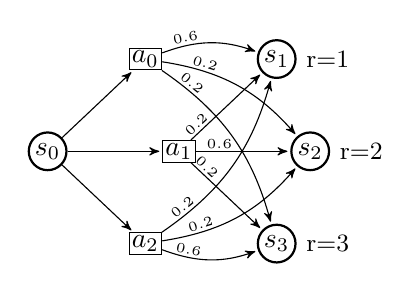
\begin{tikzpicture}[>=stealth',
	shorten > = 1pt,
	node distance = 1.2cm,
	el/.style = {inner sep=1pt, align=left, sloped},
	every label/.append style = {font=\tiny}
	]
	\node (q0) [state,thick,inner sep=1pt,minimum size=0.5pt ]     {$s_0$};
	
	\node (a0) [state,rectangle,above right=of q0,inner sep=1pt,minimum size=0.5pt ]   {$a_0$};
	\node (a1) [state,rectangle,right=of q0,inner sep=1pt,minimum size=0.5pt]   {$a_1$};
	\node (a2) [state,rectangle,below right=of q0,inner sep=1pt,minimum size=0.5pt]   {$a_2$};
	
	\node[label=right:{\small r=1}] (q1) [state,thick,right=of a0,inner sep=1pt,minimum size=0.5pt]   {$s_1$};
	\node[label=right:{\small r=2}] (q2) [state,thick,right=of a1,inner sep=1pt,minimum size=0.5pt]   {$s_2$};
	\node[label=right:{\small r=3}] (q3) [state,thick,right=of a2,inner sep=1pt,minimum size=0.5pt]   {$s_3$};
	
	\path[->] 
	(q0)  edge  (a0)
	(q0)  edge  (a1)
	(q0)  edge  (a2)
	
	(a0)  edge [bend right=-20]  node[el,above, font=\tiny, pos=0.25]  {$0.6$}   (q1)
	(a0)  edge [bend right=-20]  node[el,above, font=\tiny, pos=0.25]  {$0.2$}   (q2)
	(a0)  edge [bend right=-20]  node[el,above, font=\tiny, pos=0.15]  {$0.2$}   (q3)
	
	(a1)  edge   node[el,above, font=\tiny, pos=0.15]  {$0.2$}   (q1)
	(a1)  edge   node[el,above, font=\tiny, pos=0.25]  {$0.6$}   (q2)
	(a1)  edge   node[el,above, font=\tiny, pos=0.15]  {$0.2$}   (q3)
	
	(a2)  edge [bend left=-20]  node[el,above, font=\tiny, pos=0.15]  {$0.2$}   (q1)
	(a2)  edge [bend left=-20]  node[el,above, font=\tiny, pos=0.25]  {$0.2$}   (q2)
	(a2)  edge [bend left=-20]  node[el,above, font=\tiny, pos=0.25]  {$0.6$}   (q3);
	\end{tikzpicture}
	\caption{Simple MDP with one non-terminal state, three actions leading to three terminal states with different transition probabilities} \label{fig:SingleState}
\end{figure}

\section{Empirical Evaluation} \label{sec:experiments}

In this section, we evaluate the estimated returns over episodes
computed by Bayes UCRL and OFVF empirically. We assume a true model of
each problem and generate a number of simulated data sets for the
known distribution. We compute the tightest optimistic estimate for
the optimal return and compare it with the optimal return for the true
model. To judge the performance of the methods, we evaluate both the
absolute error of the worst case estimates from optimal, as well as the
average case estimate from optimal.

We compare our results with Bayes-UCRL and PSRL algorithms. We omit UCRL from comparison because it performs too poorly compared to other methods. PSRL does not construct any explicit plausibility set. Rather, it is a stochastically optimistic algorithm and it proceeds in a manner similar to Thompson sampling. PSRL samples a single statistically plausible MDP in proportion to the likelihood from the posterior. Optimism at each state-action independently makes OFU algorithms far too optimistic. PSRL can overcome this problem~\cite{Osband2016} and outperforms all OFU algorithms including OFVF in average case performance. But as we will see in the experiments, OFVF performs robustly in the worst case scenario and outperforms all other methods.

We first compare the methods in a simplified setting in which we
consider the problem of estimating the value of a single state from a
Bellman update. We then evaluate the methods on different problems
involving challenging exploration in full MDP setup.

\begin{figure}
	\begin{center}
		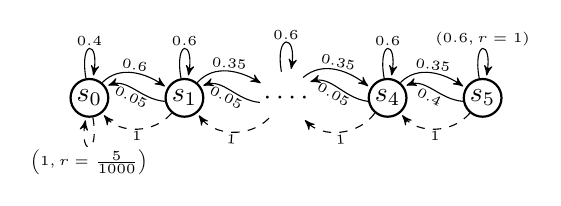
\begin{tikzpicture}[>=stealth',
		shorten > = 1pt,
		node distance = 0.7cm,
		el/.style = {inner sep=1pt, align=left, sloped},
		every label/.append style = {font=\tiny}
		]
		\node (q0) [state,thick,inner sep=1pt,minimum size=0.5pt ]     {$s_0$};
		\node (q1) [state,thick,right=of q0,inner sep=1pt,minimum size=0.5pt]   {$s_1$};
		\node (q2) [state,line width=0pt, draw=white,right=of q1,inner sep=1pt,minimum size=0.5pt]   {$\cdots\cdot$};
		\node (q4) [state,thick,right=of q2,inner sep=1pt,minimum size=0.5pt]   {$s_4$};
		\node (q5) [state,thick,right=of q4,inner sep=1pt,minimum size=0.5pt]   {$s_5$};
		
		\path[->] 
		(q0)  edge [in=260,out=280,loop, dashed] node[el,below, font=\tiny] {$\Big(1,r=\frac{5}{1000}\Big)$}   (q0)
		(q0)  edge [in=80,out=100,loop] node[el,above, font=\tiny] {$0.4$}                    (q0)
		
		(q1)  edge [in=80,out=100,loop] node[el,above, font=\tiny] {$0.6$}                    (q1)
		(q0)  edge [out=60, bend right=-50, in=150]  node[el,above, font=\tiny]  {$0.6$}      (q1)
		(q1)  edge [out=90,bend left=10, in=215]  node[el,below, font=\tiny]  {$0.05$}        (q0)
		(q1)  edge [bend left=50, dashed]  node[el,below, font=\tiny]  {$1$}                  (q0)
		
		(q2)  edge [in=80,out=100,loop] node[el,above, font=\tiny] {$0.6$}                    (q2)
		(q1)  edge [out=60, bend right=-50, in=150]  node[el,above, font=\tiny]  {$0.35$}     (q2)
		(q2)  edge [out=90,bend left=10, in=215]  node[el,below, font=\tiny]  {$0.05$}        (q1)
		(q2)  edge [bend left=50, dashed]  node[el,below, font=\tiny]  {$1$}                  (q1)
		
		(q4)  edge [in=80,out=100,loop] node[el,above, font=\tiny] {$0.6$}                    (q4)
		(q2)  edge [out=60, bend right=-50, in=150]  node[el,above, font=\tiny]  {$0.35$}     (q4)
		(q4)  edge [out=90,bend left=10, in=215]  node[el,below, font=\tiny]  {$0.05$}        (q2)
		(q4)  edge [bend left=50, dashed]  node[el,below, font=\tiny]  {$1$}                  (q2)
		
		(q5)  edge [in=80,out=100,loop] node[el,above, font=\tiny] {$(0.6, r=1)$}                    (q5)
		(q4)  edge [out=60, bend right=-50, in=150]  node[el,above, font=\tiny]  {$0.35$}     (q5)
		(q5)  edge [out=90,bend left=10, in=215]  node[el,below, font=\tiny]  {$0.4$}        (q4)
		(q5)  edge [bend left=50, dashed]  node[el,below, font=\tiny]  {$1$}                  (q4);
		
		\end{tikzpicture}
	\end{center}
	\caption{RiverSwim problem with six states $(s_0,\ldots,s_5)$ and 2 actions (left- dashed arrow, right- solid arrow)} \label{fig:RiverSwim}
\end{figure}

\begin{figure}
	\begin{center}
		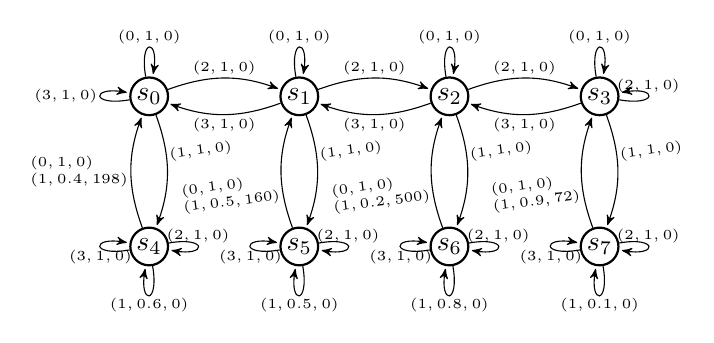
\begin{tikzpicture}[>=stealth',
		shorten > = 1pt,
		node distance = 1.4cm,
		el/.style = {inner sep=1pt, align=left, sloped},
		every label/.append style = {font=\tiny}
		]
		\node (q0) [state,thick,inner sep=1pt,minimum size=0.5pt ]     {$s_0$};
		\node (q4) [state,thick,below=of q0,inner sep=1pt,minimum size=0.5pt ]     {$s_4$};
		
		\node (q1) [state,thick,right=of q0,inner sep=1pt,minimum size=0.5pt]   {$s_1$};
		\node (q5) [state,thick,below=of q1,inner sep=1pt,minimum size=0.5pt]   {$s_5$};
		
		\node (q2) [state,thick,right=of q1,inner sep=1pt,minimum size=0.5pt]   {$s_2$};
		\node (q6) [state,thick,below=of q2,inner sep=1pt,minimum size=0.5pt]   {$s_6$};
		
		\node (q3) [state,thick,right=of q2,inner sep=1pt,minimum size=0.5pt]   {$s_3$};
		\node (q7) [state,thick,below=of q3,inner sep=1pt,minimum size=0.5pt]   {$s_7$};
		
		\path[->]
		%self loop to q0
		(q0)  edge [in=170,out=190,loop] node[el,left, rotate=-90, font=\fontsize{2}{2.5}\selectfont] {$(3,1,0)$}   (q0)
		(q0)  edge [in=80,out=100,loop] node[el,above, font=\fontsize{2}{2.5}\selectfont] {$(0,1,0)$}                    (q0)
		
		%transition below q0
		(q0)  edge [bend right=-20]  node[el,right, rotate=90, font=\fontsize{2}{2.5}\selectfont, pos=0.35]  {$(1,1,0)$}      (q4)
		(q4)  edge [bend left=20]  node[el,left, rotate=-90, font=\fontsize{2}{2.5}\selectfont]  {$(0,1,0)$\\$(1,0.4,198)$}        (q0)
		
		%transition right q0
		(q1)  edge [in=80,out=100,loop] node[el,above, font=\fontsize{2}{2.5}\selectfont] {$(0,1,0)$}                    (q1)
		(q0)  edge [bend right=-20]  node[el,above, font=\fontsize{2}{2.5}\selectfont]  {$(2,1,0)$}      (q1)
		(q1)  edge [bend left=20]  node[el,below, font=\fontsize{2}{2.5}\selectfont]  {$(3,1,0)$}        (q0)
		%(q1)  edge [bend left=50, dashed]  node[el,below, font=\tiny]  {$1$}                  (q0)
		
		(q1)  edge [bend right=-20]  node[el,right, rotate=90, font=\fontsize{2}{2.5}\selectfont, pos=0.35]  {$(1,1,0)$}      (q5)
		(q5)  edge [bend left=20]  node[el,left, rotate=90, font=\fontsize{2}{2.5}\selectfont, pos=0.35]  {$(0,1,0)$\\$(1,0.5,160)$}        (q1)
		
		(q2)  edge [in=80,out=100,loop] node[el,above, font=\fontsize{2}{2.5}\selectfont] {$(0,1,0)$}                    (q2)
		(q1)  edge [bend right=-20]  node[el,above, font=\fontsize{2}{2.5}\selectfont]  {$(2,1,0)$}     (q2)
		(q2)  edge [bend left=20]  node[el,below, font=\fontsize{2}{2.5}\selectfont]  {$(3,1,0)$}        (q1)
		%(q2)  edge [bend left=50, dashed]  node[el,below, font=\tiny]  {$1$}                  (q1)
		
		(q2)  edge [bend right=-20]  node[el,right, rotate=90, font=\fontsize{2}{2.5}\selectfont, pos=0.35]  {$(1,1,0)$}      (q6)
		(q6)  edge [bend left=20]  node[el,left, rotate=90, font=\fontsize{2}{2.5}\selectfont, pos=0.35]  {$(0,1,0)$\\$(1,0.2,500)$}        (q2)
		
		(q3)  edge [in=80,out=100,loop] node[el,above, font=\fontsize{2}{2.5}\selectfont] {$(0,1,0)$}                    (q3)
		(q3)  edge [in=10,out=350,loop] node[el,above, rotate=-90, font=\fontsize{2}{2.5}\selectfont] {$(2,1,0)$}   (q3)
		(q2)  edge [bend right=-20]  node[el,above, font=\fontsize{2}{2.5}\selectfont]  {$(2,1,0)$}     (q3)
		(q3)  edge [bend left=20]  node[el,below, font=\fontsize{2}{2.5}\selectfont]  {$(3,1,0)$}        (q2)
		%(q4)  edge [bend left=50, dashed]  node[el,below, font=\tiny]  {$1$}                  (q2)
		
		(q3)  edge [bend right=-20]  node[el,right, rotate=90, font=\fontsize{2}{2.5}\selectfont, pos=0.35]  {$(1,1,0)$}      (q7)
		(q7)  edge [bend left=20]  node[el,left, rotate=90, font=\fontsize{2}{2.5}\selectfont, pos=0.35]  {$(0,1,0)$\\$(1,0.9,72)$}        (q3)
		
		(q4)  edge [in=170,out=190,loop] node[el,below, rotate=-90, font=\fontsize{2}{2.5}\selectfont] {$(3,1,0)$}   (q4)
		(q4)  edge [in=260,out=280,loop] node[el,below, font=\fontsize{2}{2.5}\selectfont] {$(1,0.6,0)$}                    (q4)
		(q4)  edge [in=350,out=10,loop] node[el,above,rotate=90, font=\fontsize{2}{2.5}\selectfont] {$(2,1,0)$}                    (q4)
		
		(q5)  edge [in=170,out=190,loop] node[el,below, rotate=-90, font=\fontsize{2}{2.5}\selectfont] {$(3,1,0)$}   (q5)
		(q5)  edge [in=260,out=280,loop] node[el,below, font=\fontsize{2}{2.5}\selectfont] {$(1,0.5,0)$}                    (q5)
		(q5)  edge [in=350,out=10,loop] node[el,above,rotate=90, font=\fontsize{2}{2.5}\selectfont] {$(2,1,0)$}                    (q5)
		
		(q6)  edge [in=170,out=190,loop] node[el,below, rotate=-90, font=\fontsize{2}{2.5}\selectfont] {$(3,1,0)$}   (q6)
		(q6)  edge [in=260,out=280,loop] node[el,below, font=\fontsize{2}{2.5}\selectfont] {$(1,0.8,0)$}                    (q6)
		(q6)  edge [in=350,out=10,loop] node[el,above,rotate=90, font=\fontsize{2}{2.5}\selectfont] {$(2,1,0)$}                    (q6)
		
		(q7)  edge [in=170,out=190,loop] node[el,below, rotate=-90, font=\fontsize{2}{2.5}\selectfont] {$(3,1,0)$}   (q7)
		(q7)  edge [in=260,out=280,loop] node[el,below, font=\fontsize{2}{2.5}\selectfont] {$(1,0.1,0)$}                    (q7)
		(q7)  edge [in=350,out=10,loop] node[el,above,rotate=90, font=\fontsize{2}{2.5}\selectfont] {$(2,1,0)$}                    (q7)
		;
		
		\end{tikzpicture}
	\end{center}
	\caption{CasinoLand problem with eight states $(s_0,\ldots,s_7)$ and 3 actions (0,1,2). Transitions are shown with arrows, each labeled with (action, transition probability, reward).} \label{fig:CasinoLand}
\end{figure}

\subsection{Single-state Bellman Update} \label{ssection:single_state}

We initially consider a simple problem with one single non-terminal
state. The agent can take three different actions on that state. Each
action leads to one of three terminal states with different transition
probabilities. The value function for the terminal states are fixed
and assumed to be known. The dynamics of the MDP is shown
in~\cref{fig:SingleState}. We consider an uninformative Dirichlet
prior for the transition probabilities. We run the experiments for 100
episodes. 

\cref{fig:single_state} compares the average-case and worst-case returns computed by different methods. Note that OFVF outperforms all other methods in this simplistic setting. OFVF is able to explore in a robust way maximizing the worst-case return. As expected, PSRL outperforms all other methods in average case, but performs poorly in the worst-case scenario.

\begin{figure*}
	\centering
	\begin{minipage}[c]{.85\columnwidth}
		\centering
		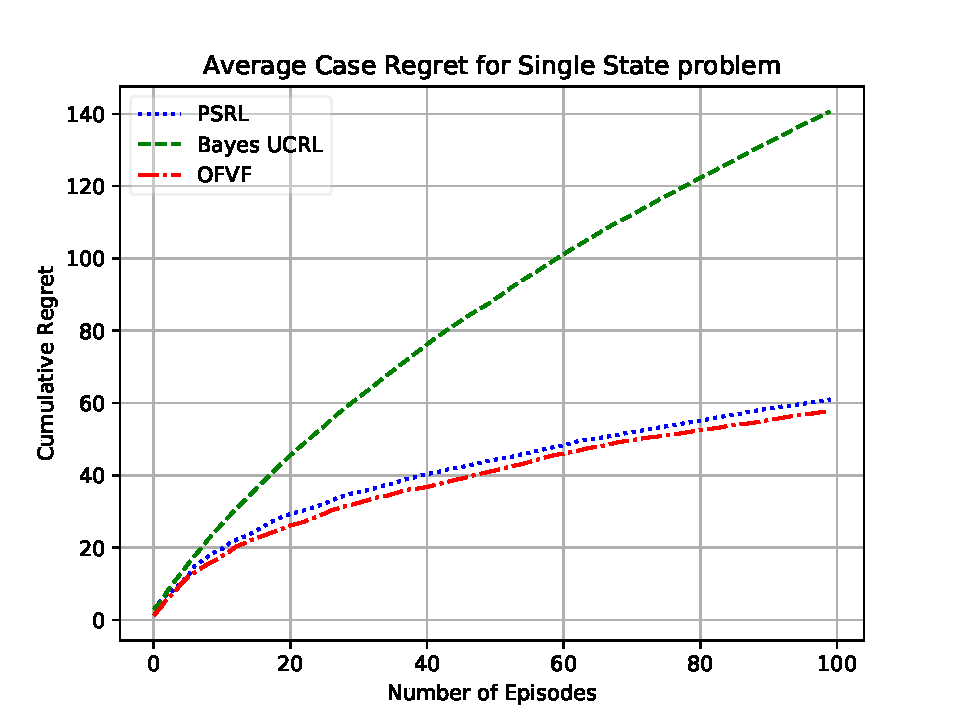
\includegraphics[width=\linewidth]{fig/SingleState_averagecase_Bayes_PSRL_OFVF.pdf}\\
	\end{minipage}%
	\begin{minipage}[c]{.85\columnwidth}
		\centering
		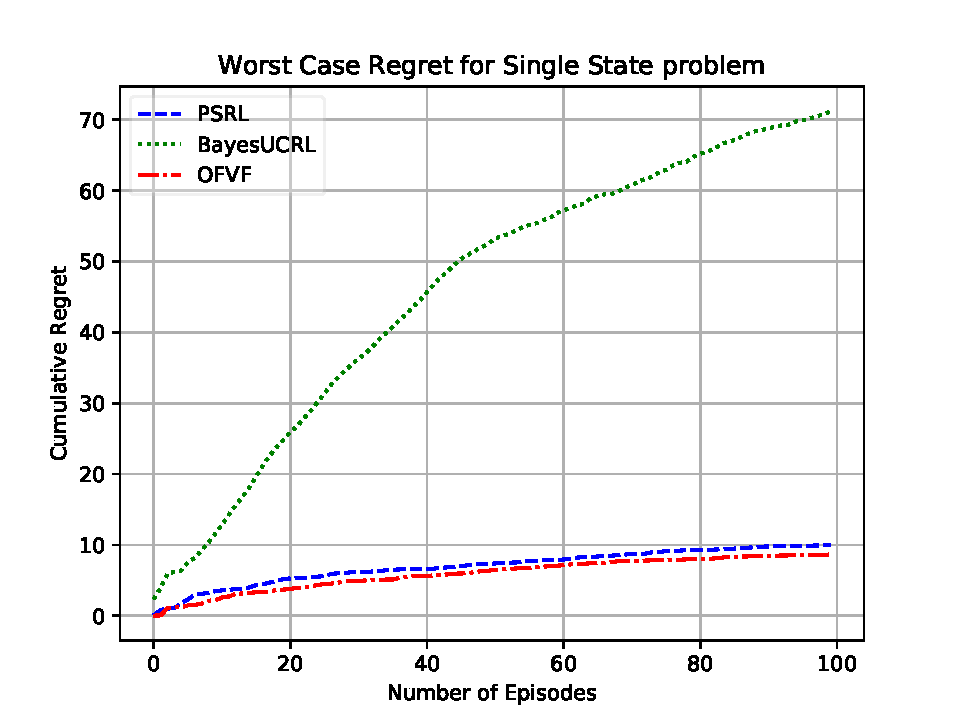
\includegraphics[width=\linewidth]{fig/SingleState_worstcase_Bayes_PSRL_OFVF.pdf}
	\end{minipage}%
	\caption{Cumulative regret for the single state simple problem. Left) average cumulative regret, Right) Worst-case cumulative regret.}
	\label{fig:single_state}
\end{figure*}

\begin{figure*}
	\centering
	\begin{minipage}[c]{.85\columnwidth}
		\centering
		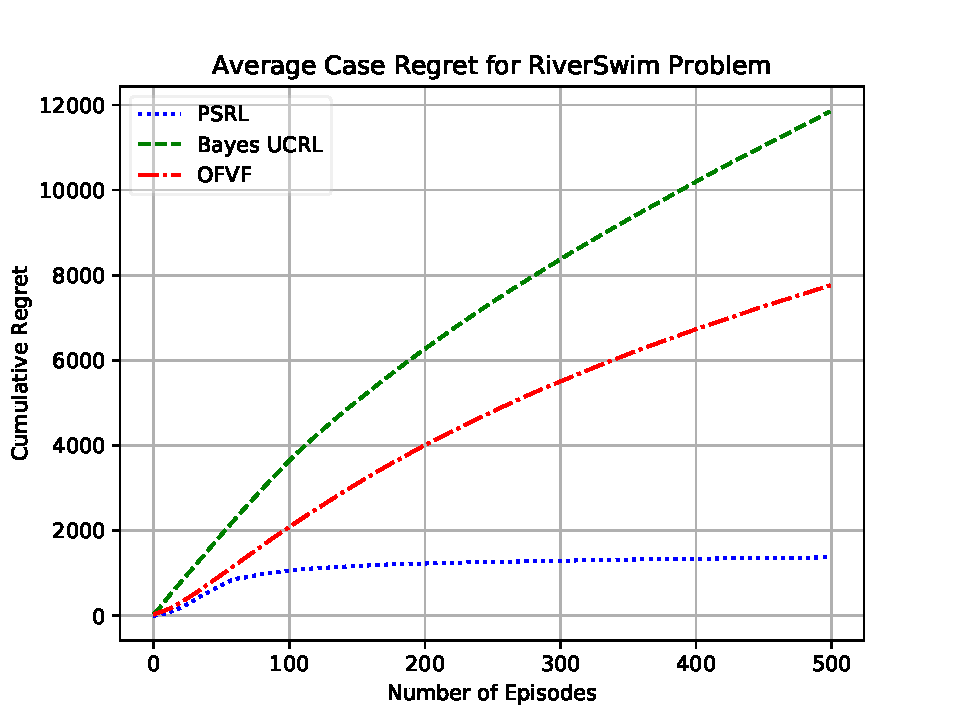
\includegraphics[width=\linewidth]{fig/RiverSwim_averagecase_Bayes_PSRL_OFVF.pdf}\\
	\end{minipage}%
	\begin{minipage}[c]{.85\columnwidth}
		\centering
		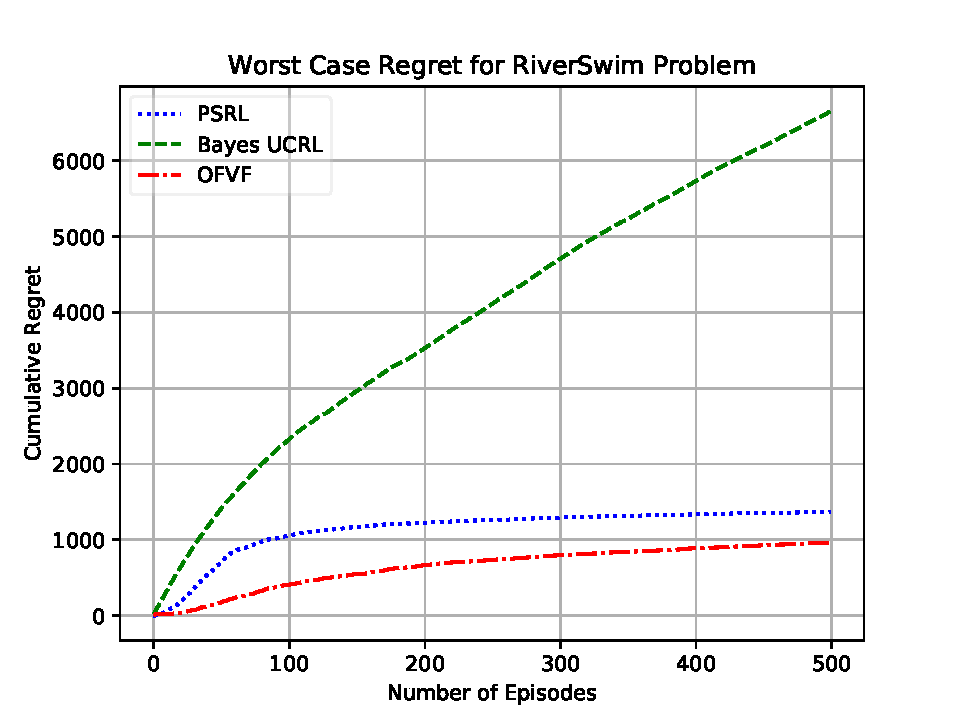
\includegraphics[width=\linewidth]{fig/RiverSwim_worstcase_Bayes_PSRL_OFVF.pdf}
	\end{minipage}%
	\caption{Cumulative regret for the RiverSwim problem. Left) average cumulative regret, Right) Worst-case cumulative regret.}
	\label{fig:riverswim}
\end{figure*}

\begin{figure*}
	\centering
	\begin{minipage}[c]{.85\columnwidth}
		\centering
		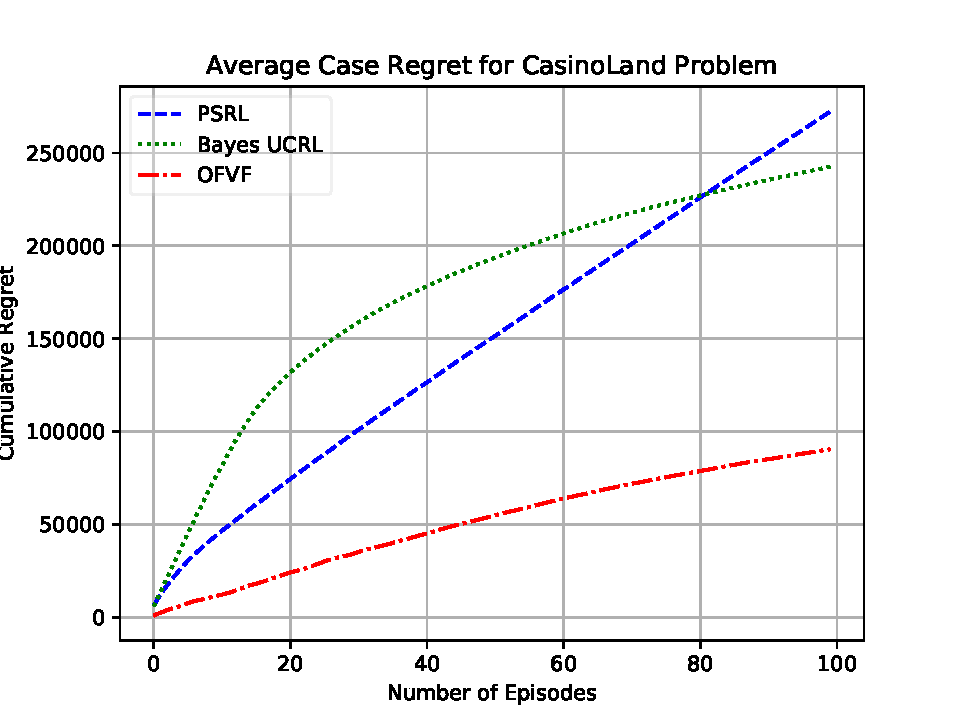
\includegraphics[width=\linewidth]{fig/casino_land_averagecase_Bayes_PSRL_OFVF.pdf}\\
	\end{minipage}%
	\begin{minipage}[c]{.85\columnwidth}
		\centering
		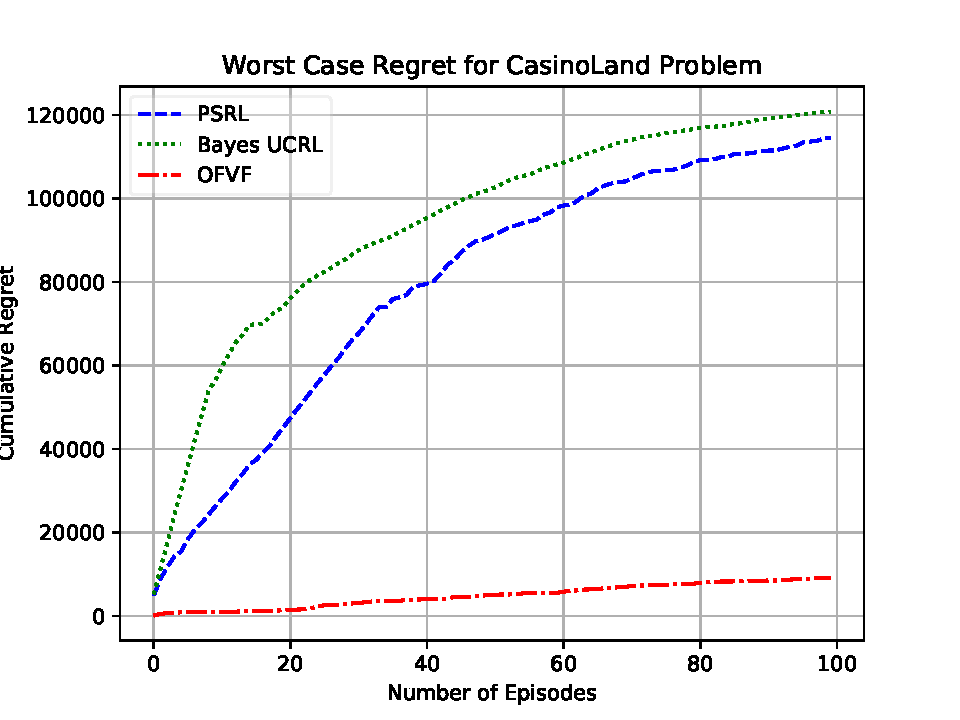
\includegraphics[width=\linewidth]{fig/casino_land__worstcase_Bayes_PSRL_OFVF.pdf}
	\end{minipage}%
	\caption{Cumulative regret for the CasinoLand problem. Left) average cumulative regret, Right) Worst-case cumulative regret.}
	\label{fig:casinoland}
\end{figure*}

\subsection{RiverSwim Problem}


We compare the performance of different methods in standard example of
RiverSwim~\citep{Osband2013, Strehl2004}. RiverSwim consists of a
chain of six states as shown in \cref{fig:RiverSwim}. The agent starts
at the left-most state $s_0$. The agent can take one of two action:
left or right. Strong current flows in the river from right to left.
Swimming left thus always successful and takes the agent to the state
on the left with probability 1. Swimming right goes against the
current and often fails. The agent receives a very small reward for
reaching leftmost state. But the rightmost state gives a much higher
reward, and the optimal policy is to swim right. Efficient exploration
is required in this problem to find the optimal policy.

We start with a uniform Dirichlet prior over the transition
probabilities. We run the experiments for 500 episodes with each
containing 100 Monte Carlo simulations. We compute the worst and
average case cumulative regrets over the episodes.
\cref{fig:riverswim} shows that, OFVF outperforms all other methods in
terms of worst-case cumulative regret.

\subsection{CasinoLand Problem}
We compare the performance of the algorithms on another challenging exploration environment, CasinoLand~\citep{Strehl2004}. CasinoLand consists of eight rooms in a two-by-four grid as shown in~\cref{fig:CasinoLand}. The transition model of the agent is shown in the picture. On the top row, the agent can move freely to any direction. Actions are less rewarding on the top row, with rewards basically zero for all the movements. On the bottom row, no horizontal movement is allowed. Taking an specific action (conceptually pulling a lever) yields a large reward with small probability. The MDP requires hard exploration because the lever with smallest probability of generating reward is the best lever to pull.

We start with a uniform Dirichlet prior over the transition
probabilities. We run the experiments for 500 episodes with each
containing 100 Monte Carlo simulations. We compute the worst and
average case cumulative regrets over the episodes.
\cref{fig:casinoland} shows that, OFVF outperforms all other methods
in terms of worst-case cumulative regret.

\subsection{Mountain Car Problem}
Next, we run experiments on the MountainCar problem from OpenAI Gym~\citep{openai}. The problem is about driving an under-powered car to the top (position=0.5) of a one-dimensional hill on the right side of the car. There is also a hill on the left side of the car. There are two actions, going left or right. The engine of the car is not strong enough, it cannot directly drive up to the hill on the right to reach the goal. But climbing the hill on the left of the car can give some momentum and that extra energy can help the car drive towards the target on the top of the right hill.

We start with a uniform Dirichlet prior for transition over the nearby states of each individual state. We compute the reference optimal solution by running Q-Learning for a very large number $(10^5)$ of episodes. We run our algorithms for hundreds of episodes each containing hundreds of consequent runs. We compare both the average-case and worst-case cumulative regret. [reference] plot shows that, OFVF outperforms all other methods in the worst case scenario.

\section{Summary and Conclusion} \label{sec:conclusion}
We presented, in this paper, a new Bayesian approach to construct the set of plausible MDPs to drive exploration. This approach has several advantages over previously used distribution free methods. Bayes-UCRL can incorporate any structural prior knowledge and it is easy to generalize the shape of the plausibility sets to other norms, not only $L_1$ norms. We proposed OFVF, a Bayesian algorithm capable of constructing plausibility sets with better shapes and sizes. Beside the fact that our proposed Bayesian methods are computationally demanding than other distribution free methods, our theoretical and experimental analysis furnished that they can pay off with much tighter robust return estimates. We showed that, OFU algorithms can be useful for robust exploration by maximizing the worst-case return.

\bibliography{marek,reazul_lib}

\newpage
\appendix
\onecolumn

\section{Technical Results} \label{app:proofs}
\subsection{Computing Bayesian Confidence Interval}

\begin{algorithm}[H]
	\KwIn{Distribution $\theta$ over $p\opt_{s,a}$, confidence level $\delta$, sample count $m$}
	\KwOut{Nominal point $\bar{p}_{s,a}$ and $L_1$ norm size $\psi_{s,a}$}
	Sample $X_1, \ldots, X_m \in \Delta^S$ from $\theta$: $X_i \sim \theta $\;
	Nominal point: $\bar{p}_{s,a} \gets (1/ m) \sum_{i=1}^m X_i $\;
	Compute distances $d_i \gets \lVert \bar{p}_{s,a} - X_i \rVert_1$ and sort \emph{increasingly}\;
	Norm size: $\psi_{s,a} \gets d_{(1-\delta)\,m}$\;
	\Return{$\bar{p}_{s,a}$ and $\psi_{s,a}$}\;
	\caption{Bayesian Confidence Interval (BCI)} \label{alg:bayes}
\end{algorithm}

\end{document}
